\documentclass[aspectratio=169]{beamer}
\usetheme{Madrid}

\usepackage{lmodern}
\usepackage[utf8]{inputenc}
\usepackage[T1]{fontenc}
\usepackage[portuguese]{babel}
\usepackage{amsmath,amssymb,bm}
\usepackage{graphicx}
\usepackage{booktabs}
\usepackage{multirow}

% bloco sem sombra: evita artefactos de renderização no Madrid
\setbeamertemplate{blocks}[rounded][shadow=false]

\graphicspath{{figures/}}

\title[HoTHP]{HoTHP: Processo de Hawkes com Codificação de Posição Rotacional Hiperbólica}
\subtitle{Extrapolação de Comprimento em Processos Temporais de Ponto}
\author[H. R. Soares]{Hugo Ramos Soares}
\institute[UFC]{Universidade Federal do Ceará \\ Orientador: César Lincoln C. Mattos e João Paulo Pordeus}
\date{2026}

\begin{document}

% Slide 1: título
\begin{frame}
  \titlepage
\end{frame}

% Sumário
\begin{frame}{Sumário}
  \tableofcontents
\end{frame}

% ============================================================
\section{Motivação}
% ============================================================

% Slide 2: sequências de eventos no mundo real
\begin{frame}{Sequências de eventos no mundo real}
  Fenômenos que ocorrem em tempo contínuo e que precisamos modelar:
  \vspace{0.4em}
  \begin{columns}[T]
    \begin{column}{0.25\textwidth}
      \centering
      \textbf{Telemetria} \\
      \small falhas em sistemas, alertas de infraestrutura
    \end{column}
    \begin{column}{0.25\textwidth}
      \centering
      \textbf{Redes sociais} \\
      \small retweets, curtidas, respostas em cascata
    \end{column}
    \begin{column}{0.25\textwidth}
      \centering
      \textbf{Saúde} \\
      \small internações, exames, prescrições de um paciente
    \end{column}
    \begin{column}{0.25\textwidth}
      \centering
      \textbf{Manutenção} \\
      \small falhas em equipamentos industriais
    \end{column}
  \end{columns}
  \vspace{0.8em}
  \begin{block}{O que há em comum?}
    Cada domínio gera uma sequência ordenada de eventos com timestamps:
    $\mathcal{S} = \{(t_1, k_1), (t_2, k_2), \ldots, (t_N, k_N)\}$
  \end{block}
\end{frame}

% Slide 3: o que queremos modelar?
\begin{frame}{O que queremos modelar?}
  Dada uma sequência de eventos passados, queremos responder:
  \begin{itemize}
    \item \textbf{Quando} ocorrerá o próximo evento?
    \item \textbf{De que tipo} será esse evento?
  \end{itemize}
  \vspace{0.5em}
  A ferramenta central é a \textbf{intensidade condicional}:
  \[
    \lambda(t \mid \mathcal{H}_t) = \lim_{dt \to 0}
      \frac{P(\text{evento em } [t, t+dt) \mid \mathcal{H}_t)}{dt}
  \]
  onde $\mathcal{H}_t$ representa todos os eventos anteriores ao instante $t$.
  \vspace{0.5em}
  \begin{block}{Objetivo do aprendizado}
    Aprender $\lambda(t)$ a partir de dados, de forma que o modelo generalize
    para sequências com comprimentos diferentes dos vistos no treinamento.
  \end{block}
\end{frame}

% Slide 4: o problema prático
\begin{frame}{O problema prático}
  \begin{columns}[T]
    \begin{column}{0.55\textwidth}
      A atenção do Transformer tem custo $O(L^2)$ em memória e tempo.
      \vspace{0.4em}
      \begin{itemize}
        \item Dobrar o comprimento da sequência quadruplica o custo.
        \item Empresas treinam em sequências curtas por restrição de recursos.
        \item Em produção, as sequências podem ser muito mais longas.
      \end{itemize}
      \vspace{0.4em}
      \textbf{Pergunta central:} é possível treinar em sequências curtas e
      obter bom desempenho em sequências longas?
    \end{column}
    \begin{column}{0.42\textwidth}
      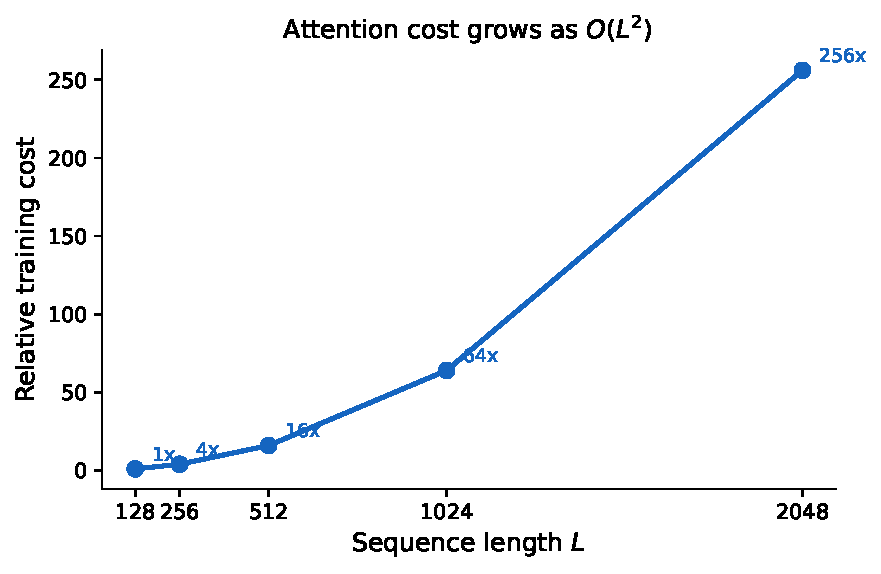
\includegraphics[width=\textwidth]{cost_curve}
    \end{column}
  \end{columns}
\end{frame}

% ============================================================
\section{Processos Temporais de Ponto}
% ============================================================

% Slide 5: o que é um PTT?
\begin{frame}{Processos Temporais de Ponto (PTT)}
  Imagine eventos que ocorrem aleatoriamente ao longo do tempo: tremores,
  publicações em redes sociais, falhas em servidores.

  \vspace{0.5em}
  Um \textbf{Processo Temporal de Ponto} é um modelo estocástico para
  esse tipo de sequência:
  \[
    \mathcal{S} = \{(t_1, k_1),\; (t_2, k_2),\; \ldots,\; (t_N, k_N)\}
  \]
  onde $t_i \in \mathbb{R}_+$ é o instante do evento e
  $k_i \in \{1, \ldots, K\}$ é o seu tipo.

  \vspace{0.5em}
  A quantidade central é a \textbf{intensidade condicional}:
  \[
    \lambda_k(t \mid \mathcal{H}_t) \;=\; \lim_{\Delta t \to 0}
      \frac{P\bigl(\text{evento do tipo } k \text{ em }
            [t,\, t{+}\Delta t) \mid \mathcal{H}_t\bigr)}{\Delta t}
  \]
  \begin{block}{}
    $\mathcal{H}_t = \{(t_i, k_i) : t_i < t\}$ é o histórico de todos os
    eventos anteriores ao instante $t$.
  \end{block}
\end{frame}

% Slide 5b: o caso mais simples -- Processo de Poisson
\begin{frame}{O caso mais simples: Processo de Poisson}
  No \textbf{Processo de Poisson Homogêneo}, a intensidade é constante:
  \[
    \lambda(t \mid \mathcal{H}_t) = \mu
  \]
  \begin{itemize}
    \item Os eventos ocorrem de forma completamente aleatória e
          \textbf{sem memória}: o passado não influencia o futuro.
    \item Os intervalos entre eventos seguem uma distribuição exponencial.
    \item É o ponto de partida clássico para modelar contagens ao longo
          do tempo.
  \end{itemize}
  \vspace{0.4em}
  \begin{alertblock}{Limitação}
    Processos reais não são sem memória. Um terremoto aumenta a
    probabilidade de réplicas nas horas seguintes. Um post viral gera
    uma cascata de reações. O Processo de Poisson não capta isso.
  \end{alertblock}
\end{frame}

% Slide 6: o processo de Hawkes
\begin{frame}{O Processo de Hawkes}
  O Processo de Hawkes estende o Processo de
  Poisson adicionando \textbf{auto-excitação}: cada evento passado
  contribui para aumentar a intensidade no presente.
  \[
    \lambda(t) = \mu + \sum_{t_i < t} \varphi(t - t_i)
  \]
  \begin{itemize}
    \item $\mu$: taxa de base (intensidade estacionária).
    \item $\varphi(t - t_i)$: função de excitação, tipicamente exponencial:
          $\varphi(\tau) = \alpha e^{-\beta \tau}$.
    \item Cada evento causa um salto em $\lambda$ que decai com taxa $\beta$.
  \end{itemize}
  \begin{block}{Analogia intuitiva}
    Terremotos: um abalo principal aumenta a probabilidade de réplicas,
    que por sua vez podem gerar novas réplicas.
  \end{block}
\end{frame}

% Slide 7: ilustração
\begin{frame}{Ilustração do Processo de Hawkes}
  \begin{figure}
    \centering
    
\includegraphics[width=\textwidth, height=0.62\textheight, keepaspectratio]{hawkes_illustration}
    \caption{Processo de Hawkes multivariado com dois tipos de eventos.
             Cada evento causa um salto em $\lambda(t)$, que decai
             exponencialmente.}
  \end{figure}
\end{frame}

% Slide 8: como treinar?
\begin{frame}{Como treinar esses modelos?}
  O treinamento maximiza a verossimilhança dos dados observados.
  A função de custo é a \textbf{log-verossimilhança negativa} (NLL):
  \[
    \mathcal{L} = -\left[
      \sum_{i=1}^{N} \log \lambda(t_i)
      - \int_0^T \lambda(t) \, dt
    \right]
  \]
  \begin{itemize}
    \item Primeiro termo: penaliza modelos que atribuem baixa intensidade
          nos instantes em que eventos de fato ocorreram.
    \item Segundo termo: penaliza modelos que preveem muitos eventos em
          momentos em que não ocorreu nada.
  \end{itemize}
  Quanto menor o NLL, melhor o modelo.
\end{frame}

% Slide 9: tabela comparativa
\begin{frame}{Abordagens para modelar PTTs}
  \begin{table}
    \centering
    \begin{tabular}{llll}
      \toprule
      \textbf{Família} & \textbf{Exemplo} & \textbf{Vantagem} & \textbf{Limitação} \\
      \midrule
      Paramétrica & Hawkes exp. & Interpretável, rápido & Forma funcional fixa \\
      Baseada em LSTM & NHP & Flexível, capta dep. & Treinamento lento \\
      Baseada em Transformer & THP & Paralelizável & Custo $O(L^2)$ \\
      \bottomrule
    \end{tabular}
    \caption{Comparativo entre famílias de modelos para PTTs.}
  \end{table}
\end{frame}

% ============================================================
\section{Modelos Neurais para PTTs}
% ============================================================

% Slide 10: NHP
\begin{frame}{Neural Hawkes Process (NHP)}
  \begin{columns}[T]
    \begin{column}{0.54\textwidth}
      Mei e Eisner propuseram usar uma LSTM para
      modelar a intensidade de um PTT.
      \begin{itemize}
        \item A LSTM mantém um estado oculto $\mathbf{h}_i$ que resume os
              eventos anteriores.
        \item A intensidade é calculada a partir de $\mathbf{h}_i$ com uma
              função de ativação apropriada.
        \item Captura dependências complexas entre eventos de tipos
              diferentes.
      \end{itemize}
      \begin{block}{Limitações}
        Treinamento sequencial (não paralelizável sobre os eventos),
        gradientes instáveis em sequências longas, estado oculto de
        tamanho fixo como único resumo do histórico.
      \end{block}
    \end{column}
    \begin{column}{0.43\textwidth}
      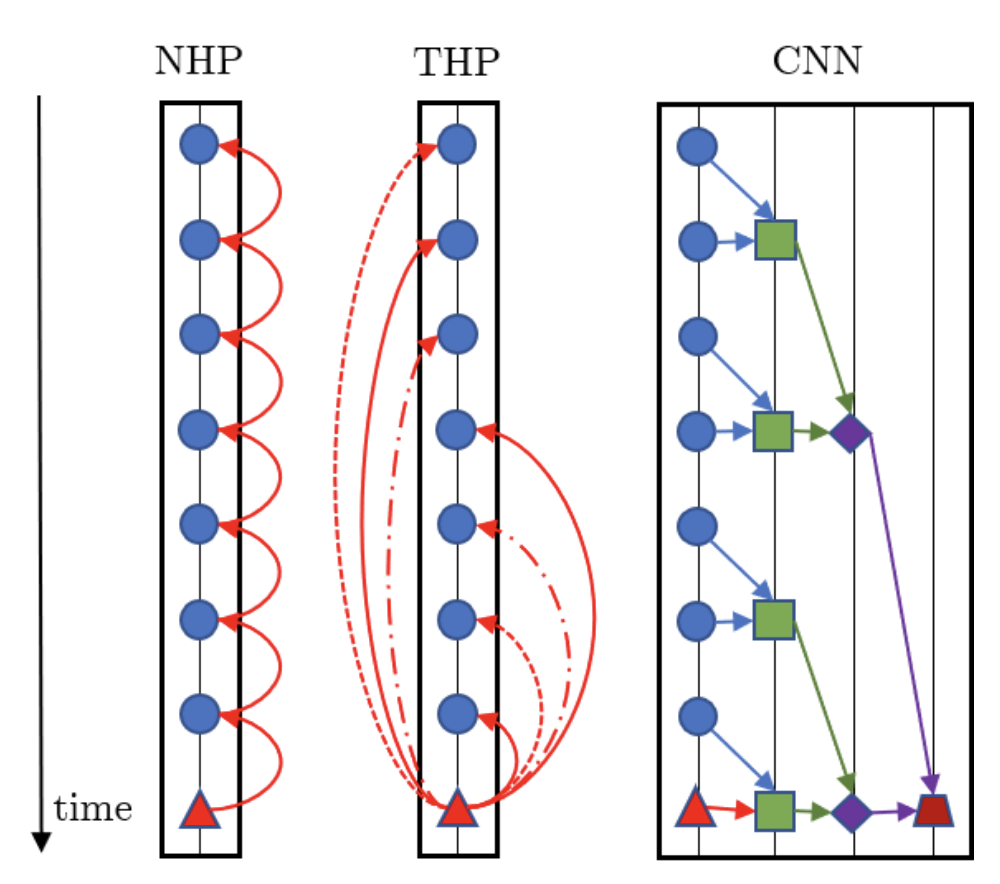
\includegraphics[width=\textwidth]{nhp_thp_comparison}
      \vspace{0.3em}
      {\small NHP processa eventos em sequência; THP consulta todos os
       eventos de uma vez.}
    \end{column}
  \end{columns}
\end{frame}

% Slide 11: Transformers
\begin{frame}{Transformers}
  \begin{columns}[T]
    \begin{column}{0.55\textwidth}
      O mecanismo de atenção permite que cada token consulte todos os
      tokens anteriores simultaneamente:
      \[
        \text{Atenção}(Q, K, V) = \text{softmax}\!\left(
          \frac{QK^\top}{\sqrt{d_k}}
        \right) V
      \]
      \begin{itemize}
        \item \textbf{Paralelizável:} todos os pares calculados de uma vez.
        \item \textbf{Atenção multi-cabeça:} diferentes dimensões capturam
              diferentes tipos de relação.
        \item O modelo não tem noção de ordem por padrão: a
              \textbf{codificação posicional} (PE) injeta essa informação
              nos embeddings de entrada.
      \end{itemize}
    \end{column}
    \begin{column}{0.4\textwidth}
      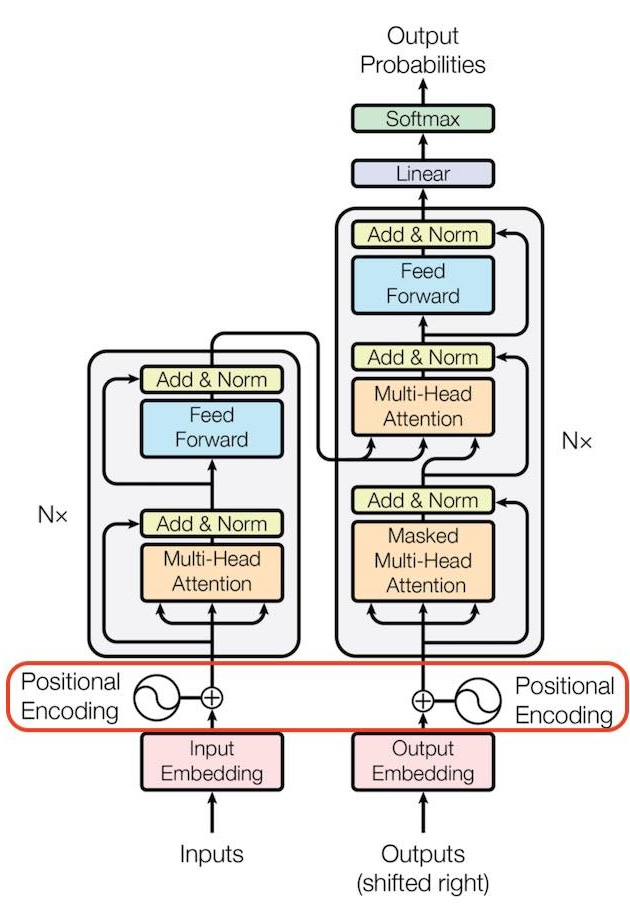
\includegraphics[width=\textwidth, height=0.8\textheight,
                       keepaspectratio]{transformer_arch}
    \end{column}
  \end{columns}
\end{frame}

% Slide 11b: embeddings + codificação posicional
\begin{frame}{Embeddings e codificação posicional}
  Cada token da entrada é representado por dois vetores somados:
  \begin{center}
    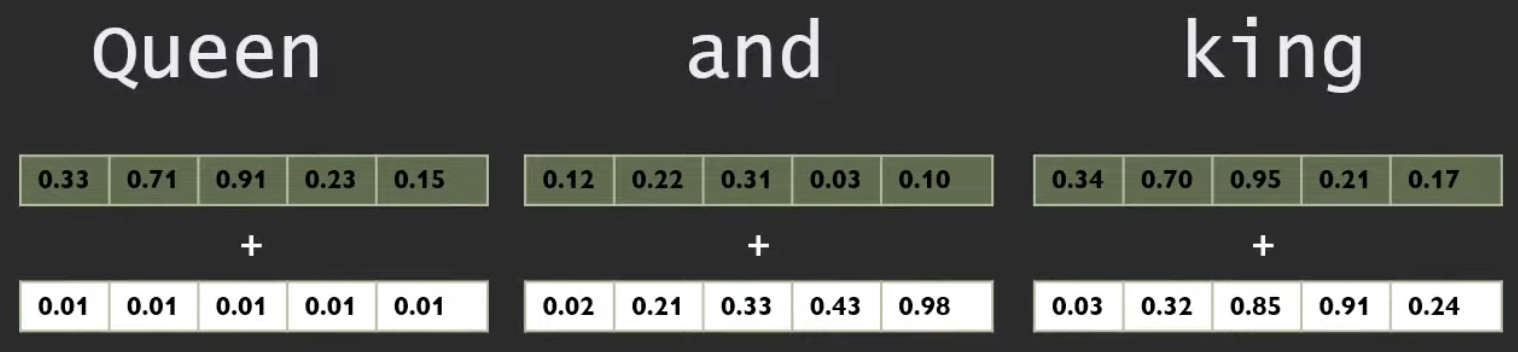
\includegraphics[width=0.72\textwidth]{pos_encoding_addition}
  \end{center}
  \begin{itemize}
    \item \textbf{Token embedding:} captura o significado semântico
          do token.
    \item \textbf{Positional encoding:} informa a posição do token na
          sequência, usando senos e cossenos de diferentes frequências.
  \end{itemize}
  \vspace{0.2em}
  {\small A mesma ideia aparece no THP: o embedding do tipo de evento
   recebe uma \textbf{codificação temporal} em vez de uma codificação
   posicional discreta.}
\end{frame}

% Slide 12: THP
\begin{frame}{Transformer Hawkes Process (THP)}
  \begin{columns}[T]
    \begin{column}{0.52\textwidth}
      Zuo et al. adaptaram o Transformer
      para PTTs: cada evento $i$ recebe um embedding de tipo somado a
      uma codificação temporal sinusoidal baseada em $t_i$.
      \[
        \mathbf{e}_i = \mathbf{w}_{k_i} +
          \bigl[\sin(\omega_j\, t_i),\; \cos(\omega_j\, t_i)\bigr]_j
      \]
      \begin{itemize}
        \item Atenção causal agrega eventos passados.
        \item Supera modelos baseados em LSTM em múltiplos benchmarks.
      \end{itemize}
      \begin{alertblock}{Limitação}
        Usa $t_i$ absoluto. O mesmo padrão de eventos deslocado produz representações diferentes.
      \end{alertblock}
    \end{column}
    \begin{column}{0.45\textwidth}
      \includegraphics[width=\textwidth, height=0.68\textheight,
                       keepaspectratio]{sinusoidal_pe}
      \vspace{0.2em}
      {\small Cada dimensão do embedding oscila em uma frequência
       diferente, criando um código único para cada posição.}
    \end{column}
  \end{columns}
\end{frame}

% Slide 13: por que invariância temporal importa?
\begin{frame}{Por que invariância temporal importa?}
  \begin{columns}[T]
    \begin{column}{0.55\textwidth}
      Um bom modelo de PTT deve depender apenas das
      \textbf{diferenças de tempo} entre eventos, não dos timestamps
      absolutos.
      \vspace{0.4em}
      \begin{itemize}
        \item O padrão de excitação de um Processo de Hawkes depende de
              $\Delta t = t_i - t_j$, não de $t_i$ ou $t_j$ isoladamente.
        \item Modelos com encoding absoluto precisam reaprender o padrão
              a cada faixa de tempo.
        \item Isso limita a capacidade de generalização fora do domínio
              de treinamento.
      \end{itemize}
    \end{column}
    \begin{column}{0.42\textwidth}
      \begin{block}{Pergunta}
        Como incorporar informação temporal de forma \textbf{relativa} ao
        mecanismo de atenção?
      \end{block}
    \end{column}
  \end{columns}
\end{frame}

% ============================================================
\section{Extrapolação de Comprimento}
% ============================================================

% Slide 14: o problema em LLMs
\begin{frame}{O problema em modelos de linguagem}
  Press et al. identificaram que modelos de linguagem
  treinados em sequências de comprimento $L$ degradam quando testados em
  sequências de comprimento $> L$.
  \begin{itemize}
    \item A perplexidade cresce de forma acentuada fora do domínio de
          treinamento.
    \item Propostas como ALiBi e RoPE surgiram como respostas: ALiBi
          subtrai um viés aditivo proporcional à distância entre tokens;
          RoPE codifica posição relativa rotacionando os vetores de query
          e key antes do produto interno.
    \item A ideia central: treinar em sequências curtas e \textbf{testar em
          sequências longas} (\emph{train short, test long}).
  \end{itemize}
\end{frame}

% Slide 15: custo de treinamento
\begin{frame}{Por que não treinar em sequências longas?}
  \begin{columns}[T]
    \begin{column}{0.52\textwidth}
      O custo da atenção cresce com o \textbf{quadrado} do comprimento:
      \vspace{0.4em}
      \begin{itemize}
        \item Dobrar $L$ quadruplica o custo.
        \item Extrapolação bem-sucedida permite treinar barato e implantar
              em sequências longas.
      \end{itemize}
    \end{column}
    \begin{column}{0.45\textwidth}
      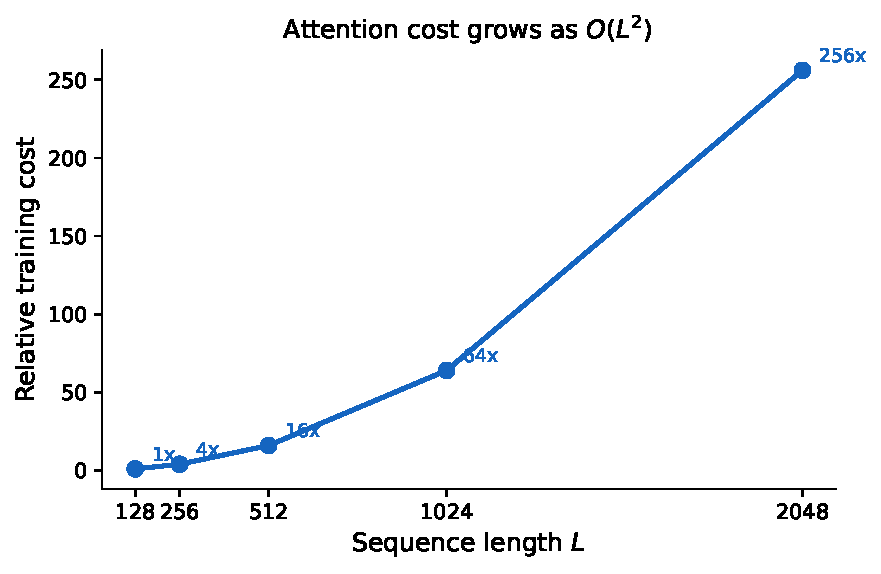
\includegraphics[width=\textwidth]{cost_curve}
    \end{column}
  \end{columns}
\end{frame}

% Slide 16: o mesmo problema em PTTs
\begin{frame}{O mesmo problema em PTTs}
  Em Processos Temporais de Ponto, a degradação tem uma forma precisa:
  \begin{itemize}
    \item O NLL aumenta quando o modelo é testado em sequências com mais
          eventos do que as vistas no treinamento.
    \item Modelos com encoding absoluto (THP) falham por construção fora
          do domínio temporal de treinamento.
    \item Modelos com encoding relativo (RoTHP) melhoram, mas o kernel
          trigonométrico é oscilatório e não decai com $|\Delta t|$,
          contradizendo a estrutura do Processo de Hawkes.
  \end{itemize}
  \begin{alertblock}{Lacuna na literatura}
    Até o RoTHP, não havia um modelo de PTT com extrapolação estável
    e alinhado com a estrutura do Processo de Hawkes.
  \end{alertblock}
\end{frame}

% Slide 17: definição formal
\begin{frame}{Protocolo \emph{Train Short, Test Long}}
  \begin{block}{Definição}
    O modelo é treinado em sequências com $N_{\text{train}}$ eventos e
    avaliado em sequências com $\alpha \cdot N_{\text{train}}$ eventos,
    onde $\alpha > 1$ é o \textbf{fator de extrapolação}.
  \end{block}
  \vspace{0.5em}
  \begin{itemize}
    \item Avaliamos $\alpha \in \{1, 2, 5, 10\}$.
    \item A métrica é o NLL médio sobre sequências de teste.
    \item Um modelo que extrapola bem deve manter NLL estável
          para valores crescentes de $\alpha$.
  \end{itemize}
\end{frame}

% ============================================================
\section{RoPE e RoTHP}
% ============================================================

% Slide 18: RoPE
\begin{frame}{Rotary Position Embedding (RoPE)}
  Su et al. propuseram codificar a posição relativa
  \textbf{rotacionando} os vetores de query e key antes do produto interno:
  \[
    \text{score}(i, j) = (R_{\theta_{t_i}} \mathbf{q})^\top (R_{\theta_{t_j}} \mathbf{k})
  \]
  \begin{itemize}
    \item $R_\theta$ é uma matriz de rotação $2 \times 2$ com frequência $\theta$.
    \item O produto interno depende apenas da \textbf{diferença} de posição
          $\theta_{t_i} - \theta_{t_j}$, garantindo invariância relativa.
    \item Custo adicional: $O(L \cdot d)$, pois cada vetor é rotacionado
          individualmente antes da atenção.
  \end{itemize}
\end{frame}

% Slide 19: RoTHP
\begin{frame}{RoTHP: RoPE para PTTs}
  Dai et al. adaptaram o RoPE para sequências de
  eventos temporais, substituindo a posição discreta por $\Delta t$:
  \begin{itemize}
    \item Os vetores $\mathbf{q}$ e $\mathbf{k}$ são rotacionados com
          ângulo determinado pelo timestamp de cada evento e pela
          frequência $\theta_\ell$ de cada dimensão.
    \item O produto interno captura a diferença temporal
          $\Delta t = t_i - t_j$ de forma relativa.
    \item O modelo passa a ser \textbf{invariante temporal}: transladar
          todos os timestamps não altera os scores de atenção.
  \end{itemize}
  \begin{block}{Avanço em relação ao THP}
    RoTHP remove a dependência de timestamps absolutos, o que é fundamental
    para generalização fora do domínio de treinamento.
  \end{block}
\end{frame}

% Slide 20: limitação do RoTHP
\begin{frame}{Limitação do RoTHP}
  \begin{columns}[T]
    \begin{column}{0.52\textwidth}
      O kernel trigonométrico do RoPE é oscilatório e \textbf{não decai}
      com $|\Delta t|$.
      \vspace{0.4em}
      \begin{itemize}
        \item Eventos distantes no tempo recebem atenção semelhante a
              eventos recentes.
        \item Isso contradiz a estrutura do Processo de Hawkes, onde a
              influência de um evento \textbf{decai exponencialmente}.
        \item O modelo não captura o viés de recência que é intrínseco
              à auto-excitação.
      \end{itemize}
    \end{column}
    \begin{column}{0.45\textwidth}
      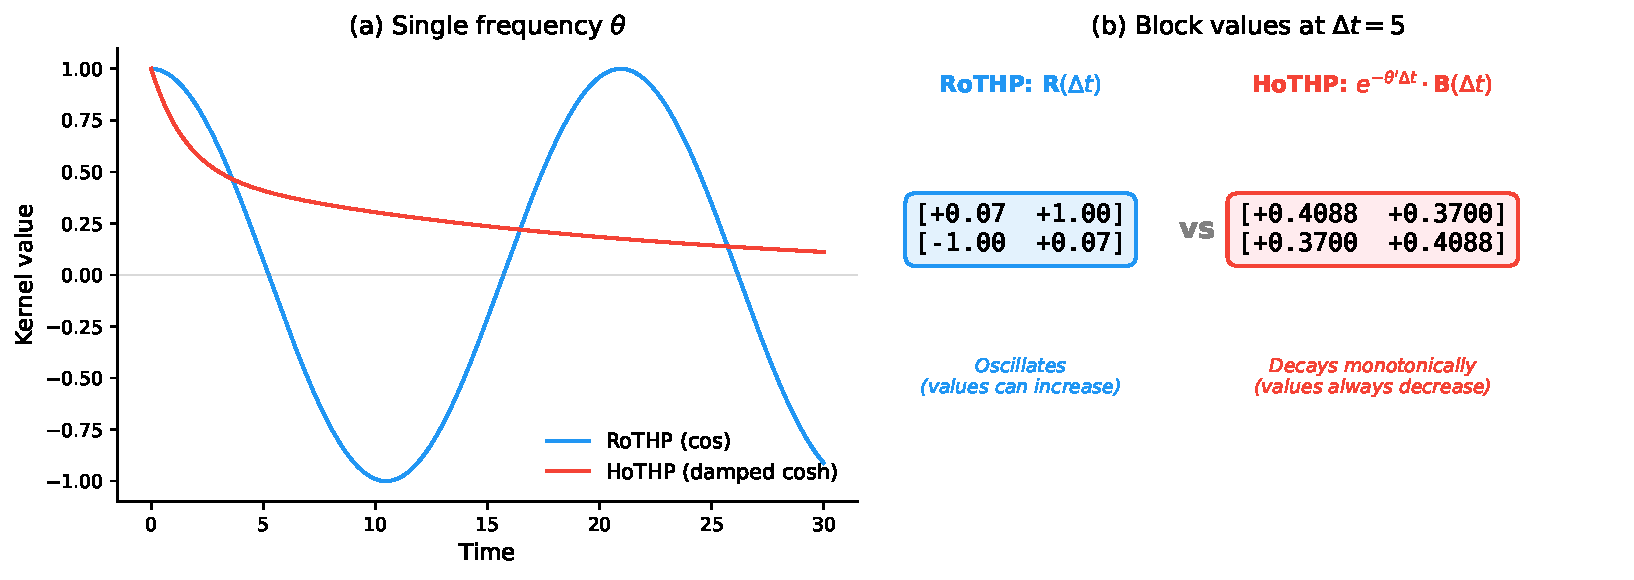
\includegraphics[width=\textwidth]{rope_vs_hope}
    \end{column}
  \end{columns}
\end{frame}

% Slide 21: comparativo de matrizes de atenção
% \begin{frame}{Perfil de atenção: RoTHP vs HoTHP}
%   \begin{figure}
%     \centering
%     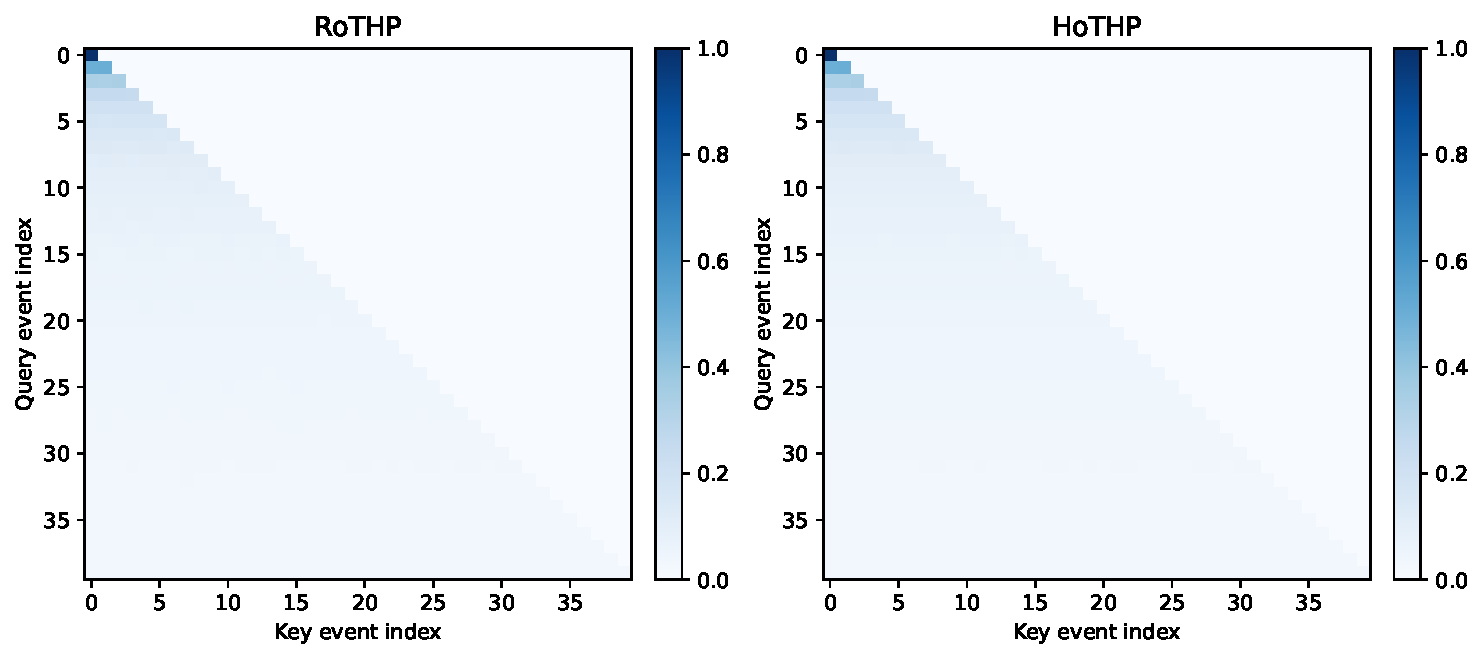
\includegraphics[width=0.88\textwidth]{attention_comparison}
%     \caption{Matrizes de peso de atenção em uma sequência de 40 eventos.
%              RoTHP: atenção dispersa sem padrão de decaimento.
%              HoTHP: atenção concentrada próxima à diagonal, decaindo
%              para eventos distantes.}
%   \end{figure}
% \end{frame}

% ============================================================
\section{HoTHP}
% ============================================================

% Slide 22: HoPE
\begin{frame}{HoPE: codificação hiperbólica para LLMs}
  Dai et al. substituíram o kernel trigonométrico do
  RoPE por funções hiperbólicas com um parâmetro de decaimento treinável
  $\theta'$:
  \begin{itemize}
    \item O kernel hiperbólico \textbf{decai} com a distância entre posições.
    \item O parâmetro $\theta'$ é aprendido durante o treinamento e
          restringido a $\theta' > \max(\theta_j)$, garantindo decaimento.
    \item Resultado: perplexidade estável em sequências mais longas que as
          vistas no treinamento, em modelos de linguagem.
  \end{itemize}
  \begin{block}{Motivação para PTTs}
    O decaimento exponencial do HoPE é exatamente o comportamento esperado
    em um Processo de Hawkes.
  \end{block}
\end{frame}

% Slide 23: o kernel hiperbólico
\begin{frame}{O kernel hiperbólico}
  O HoTHP substitui as funções trigonométricas do RoPE por funções
  hiperbólicas, mantendo a estrutura de rotação mas calculando o score
  como função de $\Delta t_{ij} = t_i - t_j$:
  \begin{align*}
    \text{score}(i,j) = \frac{e^{-|\delta|\theta'}}{\sqrt{d_k}}
      \sum_{\ell=1}^{d_k/2} \Bigl[
        &(q_{2\ell} k_{2\ell} + q_{2\ell+1} k_{2\ell+1}) \cosh(\delta\theta_\ell) \\
        +\, &(q_{2\ell} k_{2\ell+1} + q_{2\ell+1} k_{2\ell}) \sinh(\delta\theta_\ell)
      \Bigr]
  \end{align*}
  onde $\delta = \Delta t_{ij}$ e $\theta_\ell = 10000^{-2(\ell-1)/d}$.

  O fator $e^{-|\delta|\theta'}$ garante que scores entre eventos
  distantes se aproximem de zero.
\end{frame}

% Slide 24: por que hiperbólico funciona para Hawkes?
\begin{frame}{Alinhamento com o Processo de Hawkes}
  O decaimento embutido no kernel hiperbólico reproduz a estrutura
  da função de excitação $\varphi(\tau) = \alpha e^{-\beta \tau}$:
  \begin{itemize}
    \item Eventos recentes recebem maior peso de atenção.
    \item Eventos distantes têm influência próxima de zero.
    \item O parâmetro $\theta'$ é aprendido e representa a taxa de
          decaimento global do processo.
  \end{itemize}
  \begin{block}{Diferença fundamental em relação ao RoTHP}
    O RoTHP codifica posição relativa sem viés de recência. O HoTHP
    codifica posição relativa e viés de decaimento em um único
    mecanismo.
  \end{block}
\end{frame}

% Slide 25: arquitetura
% \begin{frame}{Arquitetura do HoTHP}
%   \begin{figure}
%     \centering
%     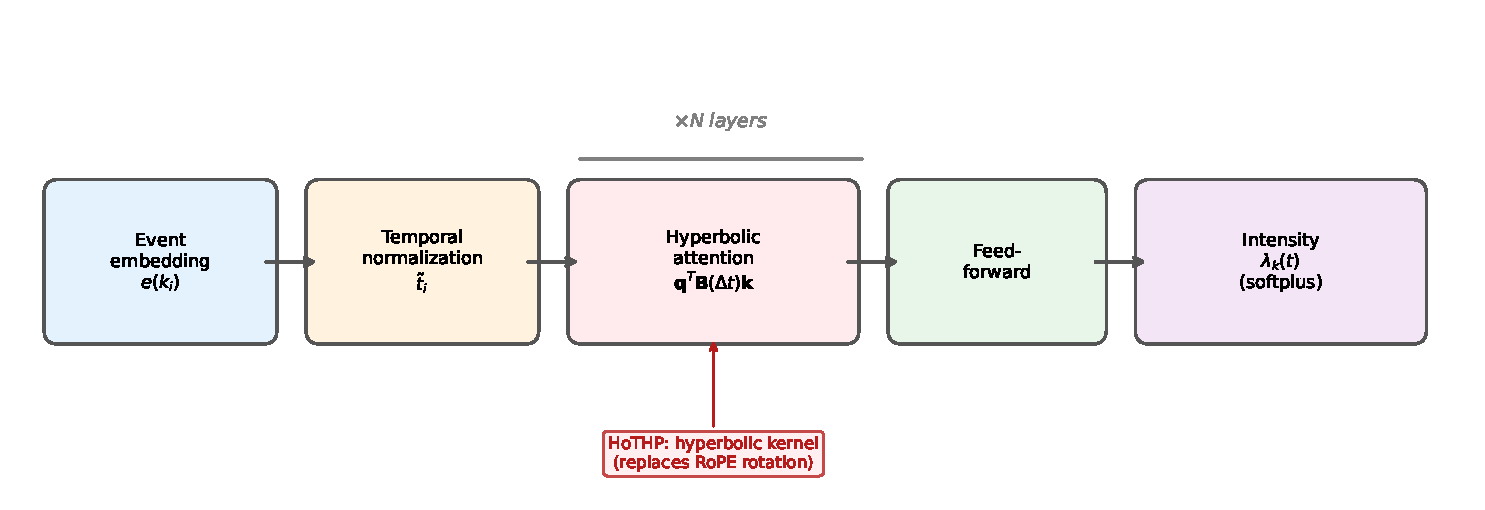
\includegraphics[width=0.80\textwidth]{architecture}
%     \caption{Arquitetura completa do HoTHP. O bloco de atenção hiperbólica
%              substitui a atenção padrão do THP e a atenção rotacional do
%              RoTHP.}
%   \end{figure}
% \end{frame}

% Slide 26: detalhe de implementação
% \begin{frame}{Detalhes de implementação}
%   \textbf{Normalização causal de timestamps}
%   \begin{itemize}
%     \item Os timestamps são normalizados de forma causal (usando apenas
%           os eventos anteriores), de modo que o gap médio seja
%           aproximadamente 1.0.
%     \item Isso evita que a escala absoluta dos timestamps influencie os
%           scores.
%   \end{itemize}
%   \vspace{0.4em}
%   \textbf{Estabilidade numérica}
%   \begin{itemize}
%     \item $\cosh(x)$ cresce como $e^x$ e pode causar overflow para
%           $\Delta t$ grande.
%     \item Solução: distribuir $e^{-|\Delta|\theta'}$ para dentro do
%           $\cosh$, reduzindo o cálculo a somas de exponenciais com
%           expoentes negativos.
%   \end{itemize}
% \end{frame}

% Slide 27: tabela resumo
\begin{frame}{Comparativo: THP, RoTHP e HoTHP}
  \begin{table}
    \centering
    \begin{tabular}{lccc}
      \toprule
      \textbf{Propriedade} & \textbf{THP} & \textbf{RoTHP} & \textbf{HoTHP} \\
      \midrule
      Invariante temporal        & Não  & Sim  & Sim \\
      Viés de decaimento         & Não  & Não  & Sim (aprendido) \\
      Extrapola para seq. longas & Não  & Parcial & Sim \\
      Parâmetros extras          & 0    & 0    & 1 ($\theta'$) \\
      \bottomrule
    \end{tabular}
    \caption{Comparativo entre THP, RoTHP e HoTHP.}
  \end{table}
\end{frame}

% ============================================================
\section{Experimentos}
% ============================================================

% Slide 28: setup experimental
\begin{frame}{Configuração experimental}
  \begin{itemize}
    \item \textbf{Dados:} sequências sintéticas geradas por Processos de
          Hawkes com dois regimes de decaimento:
          \begin{itemize}
            \item Decaimento lento ($\beta \approx 0{,}025$): influência
                  dos eventos persiste por longo período.
            \item Decaimento rápido ($\beta \approx 0{,}40$): influência
                  decai rapidamente.
          \end{itemize}
    \item \textbf{Protocolo:} treinamento em sequências de comprimento
          $N_{\text{train}}$; teste em $\alpha \cdot N_{\text{train}}$,
          com $\alpha \in \{1, 2, 5, 10\}$.
    \item \textbf{Modelos avaliados:} THP, RoTHP e HoTHP sob condições
          idênticas de treinamento.
    \item \textbf{Métrica:} NLL médio sobre as sequências de teste.
  \end{itemize}
\end{frame}

% Slide 29: perfil de atenção
\begin{frame}{Perfil de atenção teórico}
  \begin{figure}
    \centering
    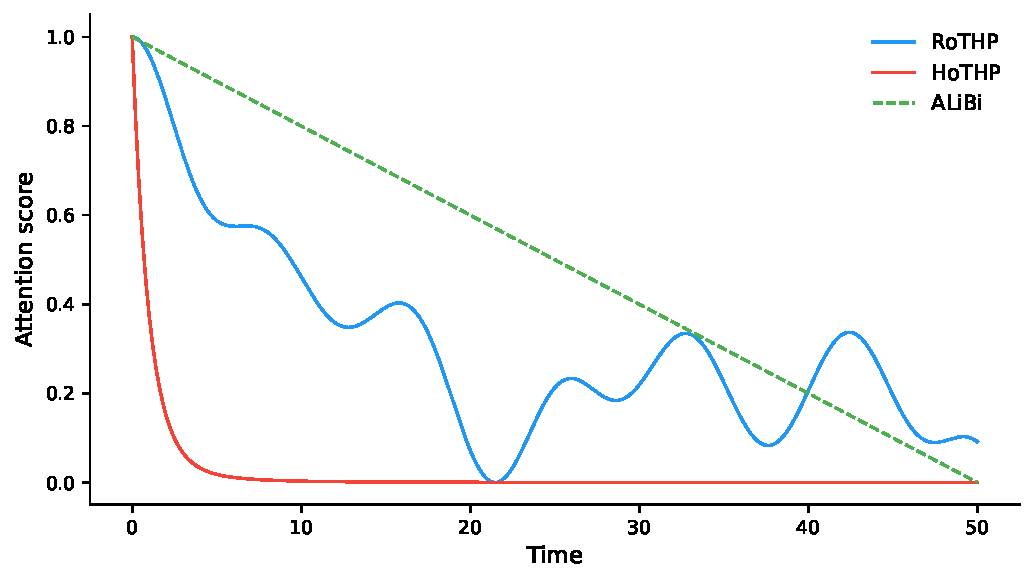
\includegraphics[width=0.82\textwidth]{attention_profile}
    \caption{Score de atenção em função de $\Delta t$.
             RoTHP oscila sem decaimento. HoTHP decai monotonicamente,
             alinhado com o comportamento teórico do Processo de Hawkes.}
  \end{figure}
\end{frame}

% Slide 30: resultado principal
\begin{frame}{Resultado principal}
  \begin{figure}
    \centering
    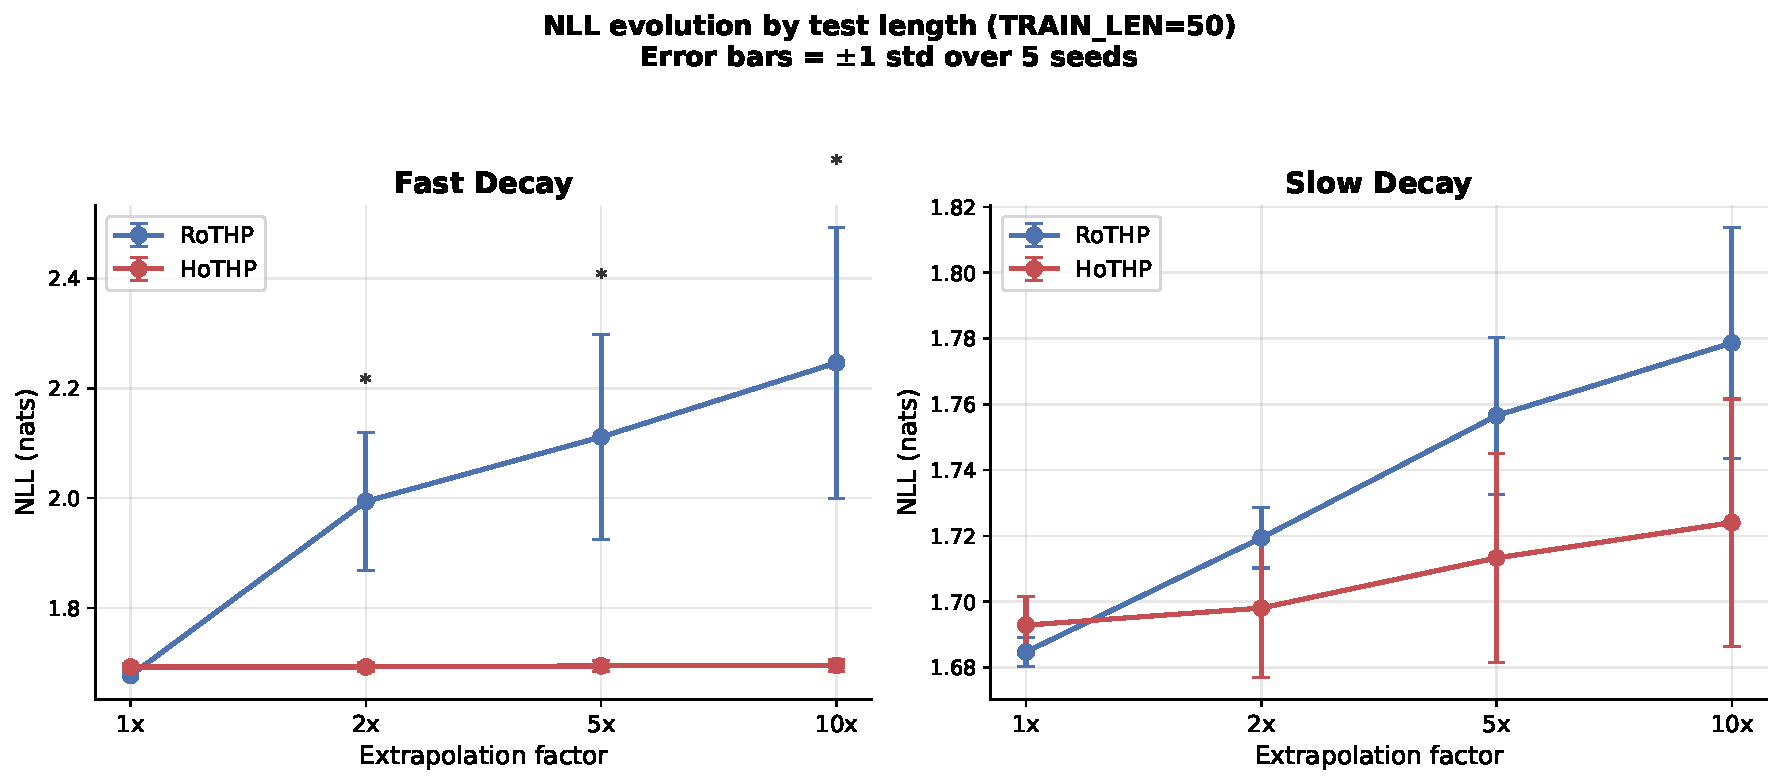
\includegraphics[width=0.88\textwidth]{main_result}
    \caption{NLL em função do fator de extrapolação $\alpha$.
             (a) Decaimento lento: modelos têm desempenho similar.
             (b) Decaimento rápido: HoTHP mantém NLL estável;
             RoTHP degrada progressivamente.}
  \end{figure}
\end{frame}

% Slide 31: alinhamento do kernel
\begin{frame}{Alinhamento do kernel aprendido}
  \begin{figure}
    \centering
    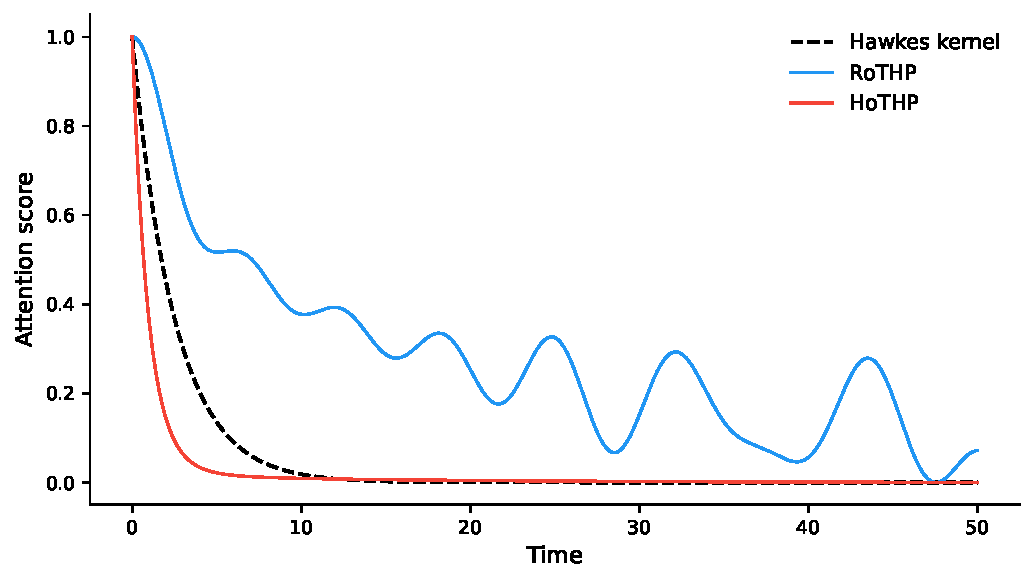
\includegraphics[width=0.82\textwidth]{kernel_alignment}
    \caption{Comparação entre o kernel aprendido pelo HoTHP e o kernel
             teórico do Processo de Hawkes. O HoTHP aprende uma forma
             funcional próxima ao decaimento exponencial teórico.}
  \end{figure}
\end{frame}

% Slide 32: tabela de resultados numéricos
\begin{frame}{Resultados numéricos}
  \begin{table}
    \centering
    \small
    \begin{tabular}{llcccc}
      \toprule
      \textbf{Dataset} & \textbf{Modelo} & $\alpha=1$ & $\alpha=2$ & $\alpha=5$ & $\alpha=10$ \\
      \midrule
      \multirow{2}{*}{Decaimento lento}
        & RoTHP  & $0{,}937$ & $1{,}005$ & $1{,}389$ & $1{,}540$ \\
        & HoTHP  & $0{,}950$ & $1{,}031$ & $1{,}403$ & $1{,}545$ \\
      \midrule
      \multirow{2}{*}{Decaimento rápido}
        & RoTHP  & $0{,}965$ & $1{,}583$ & $2{,}036$ & $2{,}362$ \\
        & HoTHP  & $0{,}958$ & $1{,}170$ & $1{,}484$ & $1{,}593$ \\
      \bottomrule
    \end{tabular}
    \caption{NLL médio por modelo e fator de extrapolação.}
  \end{table}
\end{frame}

% Slide 33: custo computacional
\begin{frame}{Custo computacional}
  \begin{table}
    \centering
    \begin{tabular}{lccc}
      \toprule
      \textbf{Modelo} & \textbf{Onde incide o custo posicional} & \textbf{Custo} & \textbf{Tempo rel. (GPU)} \\
      \midrule
      THP    & Encoding aditivo por evento  & $O(Ld)$      & $1\times$ \\
      RoTHP  & Rotação de $\mathbf{q}$, $\mathbf{k}$ por evento & $O(Ld)$ & $1\times$ \\
      HoTHP  & Kernel calculado por par de eventos & $O(L^2 d/2)$ & $3\times$ \\
      \bottomrule
    \end{tabular}
    \caption{Custo do mecanismo posicional e tempo de treino relativo medido em GPU.}
  \end{table}
  \vspace{0.3em}
  O HoTHP treina $3\times$ mais lento que o RoTHP em GPU porque o kernel
  hiperbólico precisa ser calculado para todos os $L^2$ pares de eventos,
  enquanto RoPE opera por evento individualmente.
  Em CPU, sem paralelismo de hardware, esse overhead pode ser de $10\times$ a $40\times$.
\end{frame}

% Slide 34: análise de break-even
\begin{frame}{Quando a extrapolação compensa?}
  Usando o overhead medido em GPU ($3\times$) e o custo quadrático da atenção
  ($\alpha^2$ vezes mais caro para sequências $\alpha\times$ maiores):
  \[
    \alpha^2 > 3 \implies \alpha > \sqrt{3} \approx 1{,}73
  \]
  Para sequências de teste mais que $73\%$ maiores que as de treino,
  treinar o HoTHP em sequências curtas já é mais barato do que treinar
  o RoTHP diretamente em sequências longas.
  \textbf{Benchmark em CPU (forward pass isolado):}
  \vspace{0.3em}

  {\small
  \begin{tabular}{lcccc}
    \toprule
    \textbf{Modelo} & $L=64$ & $L=128$ & $L=256$ & $L=512$ \\
    \midrule
    RoTHP  & 1,5 ms & 3,2 ms & 6,8 ms & 29,8 ms \\
    HoTHP  & 15,3 ms & 69,2 ms & 279,6 ms & 1053 ms \\
    \textit{Razão} & 10x & 21x & 41x & 35x \\
    \bottomrule
  \end{tabular}
  }

  \vspace{0.3em}
  O overhead elevado em CPU confirma que a diferença vem do $O(L^2)$ do kernel.
  Em GPU, o paralelismo reduz a razão para $3\times$.
\end{frame}

% ============================================================
\section{Conclusão}
% ============================================================

% Slide 35: contribuições
\begin{frame}{Contribuições}
  \begin{itemize}
    \item \textbf{HoTHP:} primeiro modelo de PTT com codificação de posição
          hiperbólica, combinando invariância temporal e viés de decaimento
          em um único mecanismo de atenção.
    \item O parâmetro treinável $\theta'$ aprende a taxa de decaimento
          global do processo, alinhando o modelo com a estrutura teórica
          do Processo de Hawkes.
    \item Avaliação no protocolo \emph{train short, test long} mostra NLL
          estável para fatores de extrapolação até $10\times$, enquanto
          o RoTHP degrada no regime de decaimento rápido.
    \item Código disponível no repositório da dissertação (EasyTPP).
  \end{itemize}
\end{frame}

% Slide 36: limitações e trabalhos futuros
\begin{frame}{Limitações e trabalhos futuros}
  \textbf{Limitações atuais}
  \begin{itemize}
    \item Avaliação restrita a dados sintéticos; desempenho em datasets
          reais ainda não foi verificado.
    \item Custo computacional $3\times$ maior que o RoTHP pode ser
          proibitivo para sequências muito longas.
    \item O break-even empírico foi medido apenas em CPU com forward pass
          isolado; validação em cenário de treinamento completo em GPU
          ainda não foi realizada.
  \end{itemize}
  \vspace{0.4em}
  \textbf{Trabalhos futuros}
  \begin{itemize}
    \item Avaliar em datasets reais (MIMIC, Stack Overflow, Retweet).
    \item Medir o crossover empírico entre custo de extrapolação e custo
          de treino longo.
    \item Investigar aproximações de baixo posto para reduzir o custo
          $O(L^2)$ do kernel hiperbólico.
    \item Análise teórica da convergência e das propriedades do $\theta'$
          aprendido.
  \end{itemize}
\end{frame}

% Slide 37: encerramento
\begin{frame}{Obrigado}
  \begin{center}
    \large
    \textbf{Hugo Ramos Soares} \\
    \normalsize
    \texttt{hugoramos84@gmail.com} \\[1em]
    Universidade Federal do Ceará \\
    Orientador: César Lincoln C. Mattos e João Paulo Pordeus \\[1.5em]
    \textbf{Referências principais}
  \end{center}
  \begin{itemize}
    \item Hawkes (1971) -- Processo de Hawkes original
    \item Zuo et al. (2020) -- THP
    \item Su et al. (2024) -- RoFormer/RoPE
    \item Dai et al. (2026) -- RoTHP
    \item Dai et al. (2025) -- HoPE
    \item Press et al. (2022) -- Train Short, Test Long
  \end{itemize}
\end{frame}

% Frame invisível: necessário para compilar as \cite{}, nunca renderizado
\begin{frame}<0>[noframenumbering]{}
  \bibliographystyle{plain}
  \bibliography{refs}
\end{frame}

\end{document}
